\begin{frame}{Motivación}

    \begin{block}{¿A qué vinieron?}
        \begin{itemize}
            \item Herramientas necesarias para la vida diaria, tanto académica como profesional.
            \pause
            \item No son obligatorias para la currícula, pero igualmente se esperan de nosotros.
            \pause
            \item Gastamos tiempo en tareas que deberían ser automatizables.
        \end{itemize}
    \end{block} 
    
\end{frame}

\begin{frame}{La Shell}
\begin{block}{¿Qué es?}
    \begin{itemize}
        \item Interactuamos con la computadora a través de una interfaz.
        \pause
        \item Puede ser gráfica (GUI).
            \begin{figure}
            \begin{minipage}{.5\textwidth}
              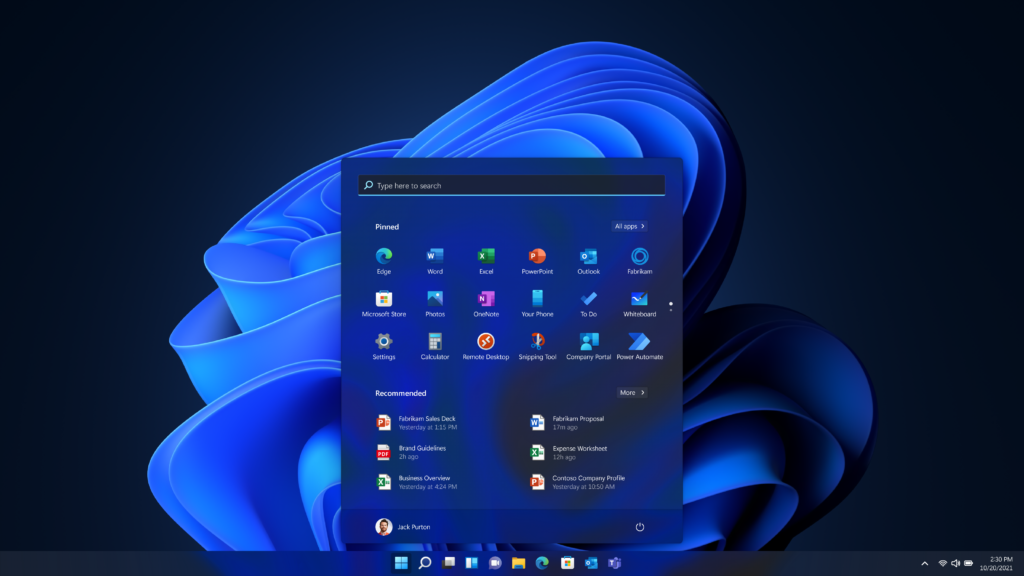
\includegraphics[width=.8\linewidth]{images/windows-gui.png}
            \end{minipage}%
            \begin{minipage}{.5\textwidth}
              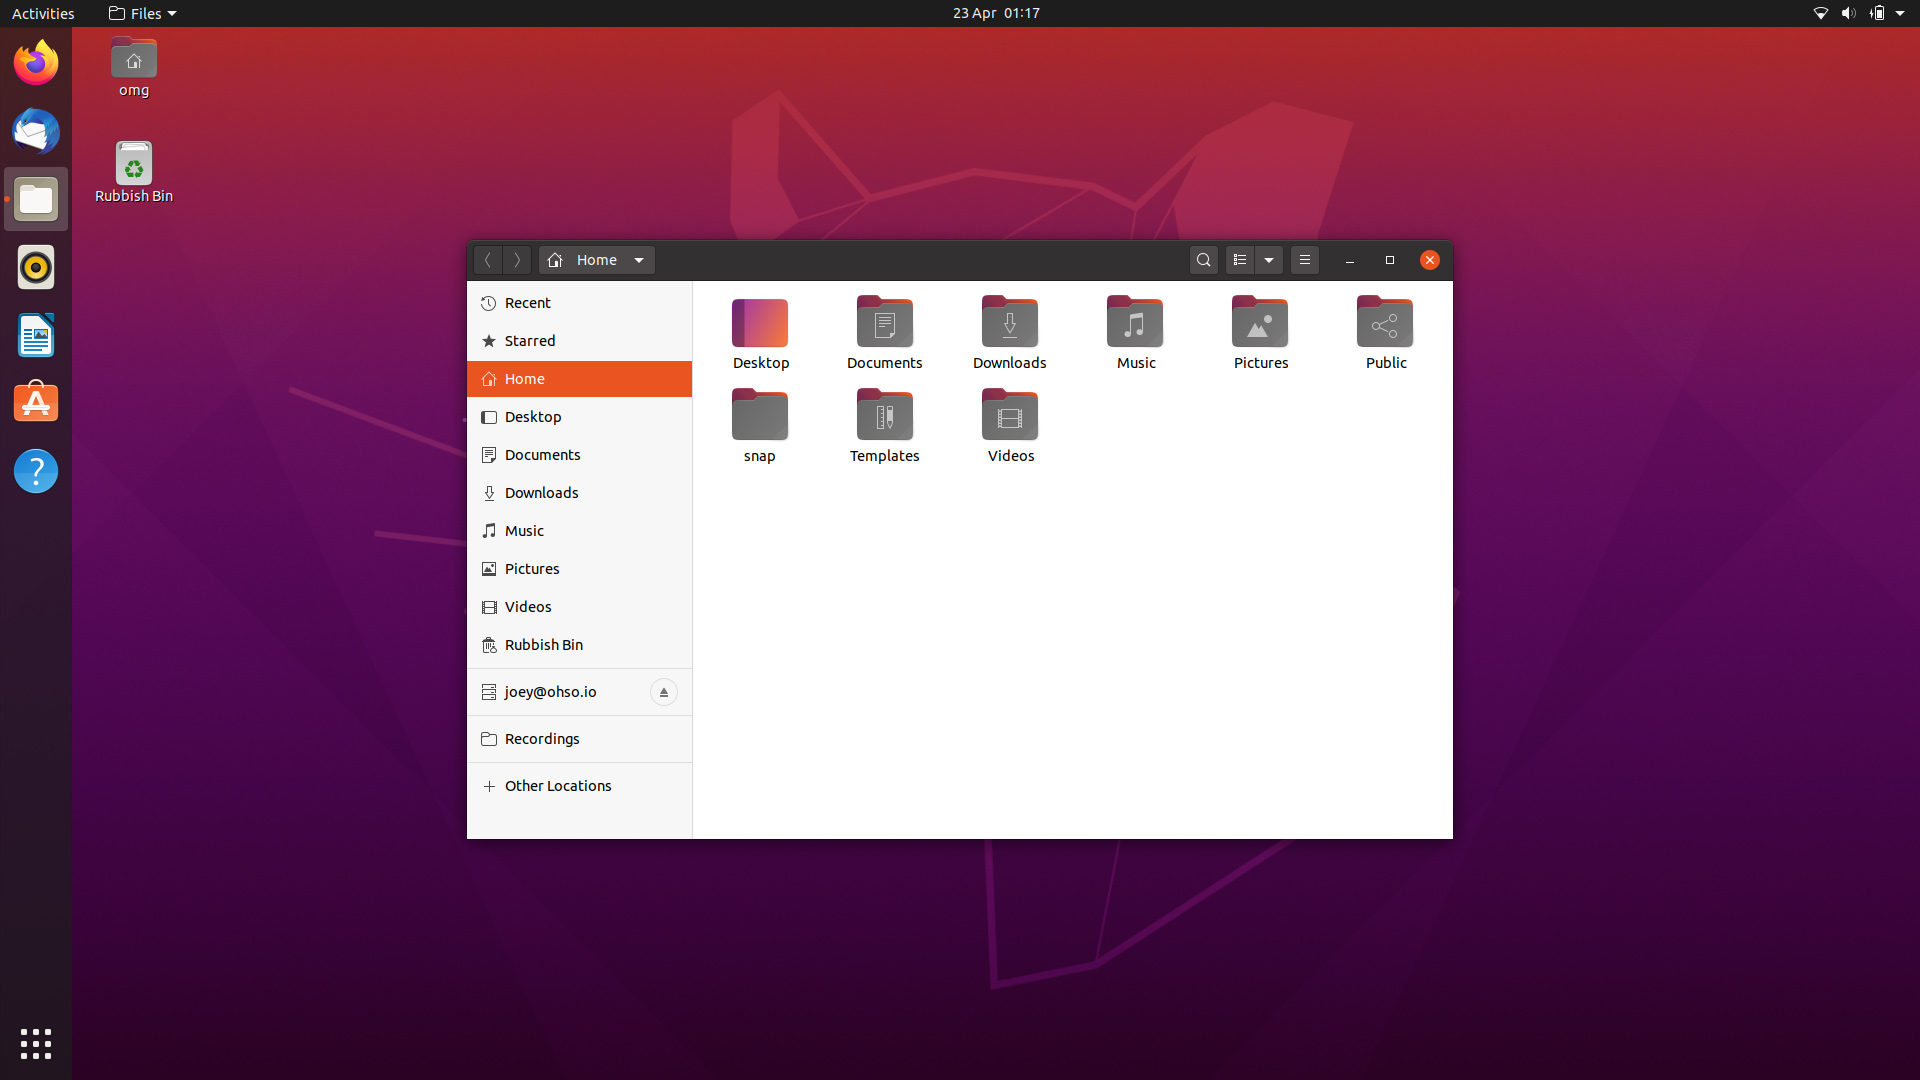
\includegraphics[width=.8\linewidth]{images/ubuntu-gui.jpg}
            \end{minipage}
            \end{figure}
        \pause
        \item O de línea de comando (CLI).
    \end{itemize}
\end{block}

\end{frame}

\begin{frame}{La Shell (2)}
    \begin{block}{¿Qué es? (2)}
        \begin{itemize}
                \item Bash AKA \textit{Bourne-Again SHell}
            \pause
            \item Para abrir un \textit{shell prompt,} necesitamos una terminal.
            \pause
        \end{itemize}
    \begin{centering}
    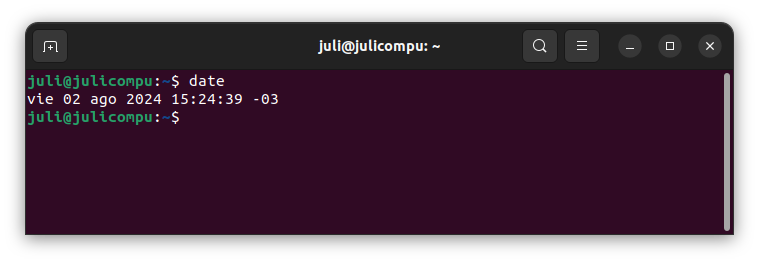
\includegraphics[height=1.5in]{images/bash-1.png}        
    \end{centering}
    \end{block}

\end{frame}

\begin{frame}{La Shell (3)}
% But how does the shell know how to find the date or echo programs? Well, the shell is a programming environment, just like Python or Ruby, and so it has variables, conditionals, loops, and functions (next lecture!). When you run commands in your shell, you are really writing a small bit of code that your shell interprets. If the shell is asked to execute a command that doesn’t match one of its programming keywords, it consults an environment variable called $PATH that lists which directories the shell should search for programs when it is given a command:
    \begin{block}{¿Cómo se usa?}
        \centering
        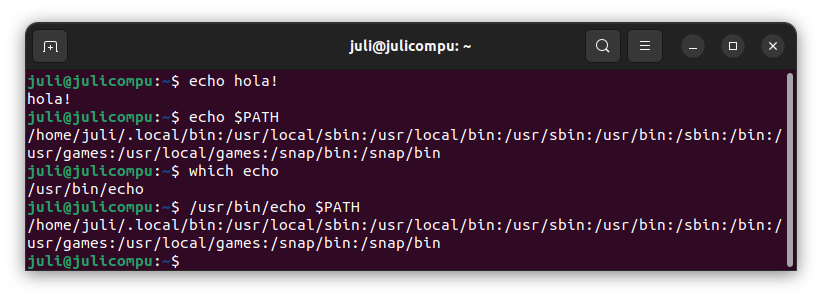
\includegraphics[width=4.5in]{images/bash-2.png}
    \end{block}
    
\end{frame}

\begin{frame}{La Shell (4)}
\begin{block}{Navegando la Shell}
        \vspace{-0.3cm}
        \centering
        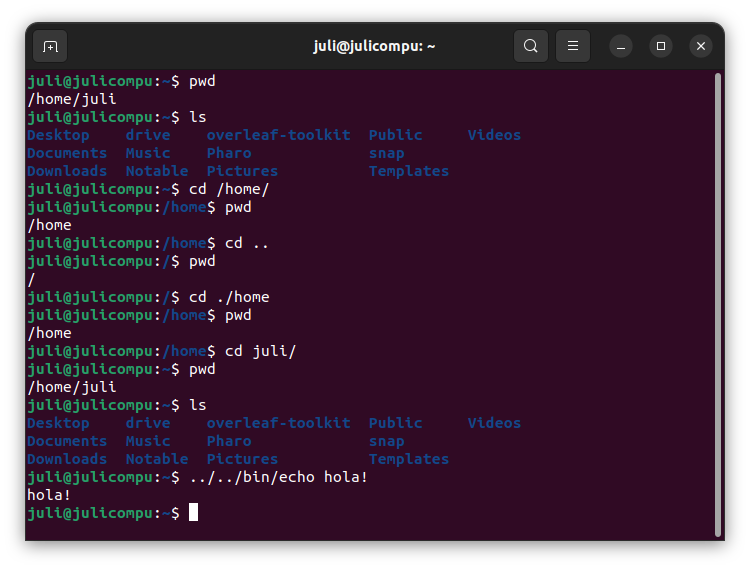
\includegraphics[width=4in]{images/bash-3.png}
\end{block}
\end{frame}

\begin{frame}{La Shell (5)}
\begin{block}{Conectando programas}
        \centering
        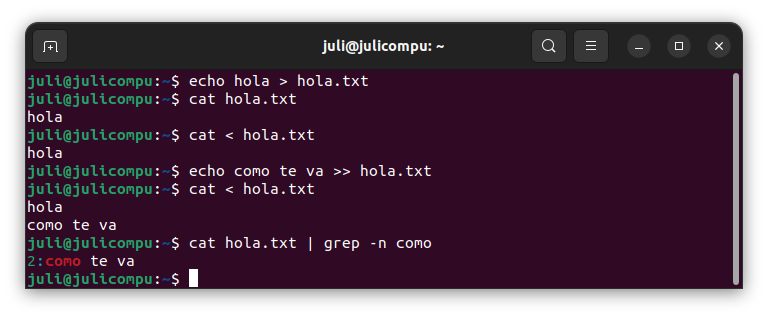
\includegraphics[width=4in]{images/bash-4.png}
\end{block}
\end{frame}

\begin{frame}{Comandos útiles}

\begin{block} {Otros ejemplos}
        \begin{itemize}
        \item touch
        \item curl
        \item nano
        \item unzip
        \item mkdir
    \end{itemize}
\end{block}

    \begin{ejercicio}{Ejercicio}
        Ejecuten \textit{man man}. ¿Qué sucedió? ¿Qué hace el programa \textit{man}?

        Úsenlo para averiguar los usos de los otros programas de más arriba.

        % explicar como avanzar o como salir?
    \end{ejercicio}
    % que bajen el archivo y le editen algo con nano
    % otro ejercicio que invoque un python usando nano, por ejemplo. o agregar comandos nuevos
    
\end{frame}

\begin{frame}{Ejercitando los comandos}

\begin{ejercicio}{Ejercicio}
    \begin{enumerate}
        \item Creen una carpeta para el taller, en donde ustedes quieran. Puede ser en el escritorio. Asegúrense de situarse dentro de ella.
        
        Ejemplo: \textit{mkdir carpeta},      
        \textit{cd carpeta}.
        
        Recuerden que la carpeta se creará en la dirección donde estén parados en la terminal. 
        \pause
        \item Usen curl para bajar el archivo en \href{https://bit.ly/taller-git-ej1}{bit.ly/taller-git-ej1}. 
        
        Ejemplo: \textit{curl -L "bit.ly/taller-git-ej1" > script.py}
        \pause
        \item Usen cat para ver el contenido del archivo. 
        
        Ejemplo: \textit{cat script.py}
        \pause
        \item Ejecuten el archivo haciendo \textit{python3 script.py}
        \pause
        \item Usando nano, cambien el comportamiento del programa para que imprima lo que ustedes quieran. 
        
        Ejemplo: \textit{nano script.py}
        \pause
        \item Vuelvan a ejecutar el archivo.
    \end{enumerate}
\end{ejercicio}
\end{frame}
